\documentclass[fleqn, a4paper, 11pt, oneside]{amsart}
%\usepackage[top = 2cm, bottom = 1cm, left = 1cm, right = 1cm]{geometry}
\usepackage{exsheets, tasks}
\usepackage{amsmath, amssymb, amsthm} %standard AMS packages
\usepackage{marginnote} %marginnotes
\usepackage{gensymb} %miscellaneous symbols
\usepackage{commath} %differential symbols
\usepackage{xcolor} %colours
\usepackage{cancel} %cancelling terms
\usepackage[free-standing-units, space-before-unit]{siunitx} %formatting units
\usepackage{tikz, pgfplots} %diagrams
\usetikzlibrary{calc, hobby, patterns, intersections, decorations.markings}
\usepackage{graphicx} %inserting graphics
\usepackage{hyperref} %hyperlinks
\usepackage{datetime} %date and time
\usepackage{ulem} %underline for \emph{}
\usepackage{xfrac} %inline fractions
\usepackage{enumerate,enumitem} %numbered lists
\usepackage{float} %inserting floats
\usepackage{circuitikz}[american voltages, american currents] %circuit diagrams
\usepackage[utf8]{inputenc}

\newcommand\numberthis{\addtocounter{equation}{1}\tag{\theequation}} %adds numbers to specific equations in non-numbered list of equations

\newcommand{\AxisRotator}[1][rotate=0]{
	\tikz [x=0.25cm,y=0.60cm,line width=.2ex,-stealth,#1] \draw (0,0) arc (-150:150:1 and 1);%
} %rotation symbols on axes

\theoremstyle{definition}
\newtheorem{example}{Example}
\newtheorem{definition}{Definition}

\theoremstyle{theorem}
\newtheorem{theorem}{Theorem}

\newcommand{\curl}{\mathrm{curl\,}}

\makeatletter
\@addtoreset{section}{part} %resets section numbers in new part
\makeatother

\renewcommand{\thesubsection}{(\arabic{subsection})}
\renewcommand{\thesection}{(\arabic{section})}

\renewcommand{\emph}{\uline}

%section headings on left
\makeatletter
\def\specialsection{\@startsection{section}{1}%
	\z@{\linespacing\@plus\linespacing}{.5\linespacing}%
	%  {\normalfont\centering}}% DELETED
	{\normalfont}}% NEW
\def\section{\@startsection{section}{1}%
	\z@{.7\linespacing\@plus\linespacing}{.5\linespacing}%
	%  {\normalfont\scshape\centering}}% DELETED
	{\normalfont\scshape}}% NEW
\makeatother

%forces newline after subsection
\makeatletter
\def\subsection{\@startsection{subsection}{3}%
	\z@{.5\linespacing\@plus.7\linespacing}{.1\linespacing}%
	{\normalfont\itshape}}
\makeatother

\settasks{counter-format = tsk[1].}

\SetupExSheets{solution/print = true}

%opening
\title{Quantum and Solid State Physics : Assignment 4}
\author
{
	Aakash Jog\\
	ID : 989323563
}
\date{\formatdate{12}{11}{2015}}

\begin{document}

\tikzset{->-/.style={decoration={
  markings,
  mark=at position #1 with {\arrow{>}}},postaction={decorate}}}

\maketitle
%\setlength{\mathindent}{0pt}

\begin{question}
	True or False:
	\begin{enumerate}
		\item Semiconductor materials at 0 \si{\kelvin} have the same structure as metals - bands either overlap or are only partially filled.
		\item In a solid, many atoms are brought close together, so that the split energy levels form essentially continuous bands.
		\item Column $\mathrm{V}$ donor levels usually lie approximately 0.95 \electronvolt below the conduction band in Si.
	\end{enumerate}
\end{question}

\begin{solution}
	\begin{enumerate}[leftmargin=*]
		\item
			False, at 0 \kelvin, semiconductors have the same structure as insulators.
		\item
			True
		\item
			False, donor levels are closer to the $E_C$ and not closer to $E_V$, as suggested by the given energy difference.
	\end{enumerate}
\end{solution}

\begin{question}
	The following diagrams illustrate, for 3 different materials, an electron in the conduction band recombining with a hole in the valence band and emitting a photon of energy $E_{\text{photon}} = E_g$, where $E_g$ is the band gap energy.
	\begin{figure}[H]
		\centering
		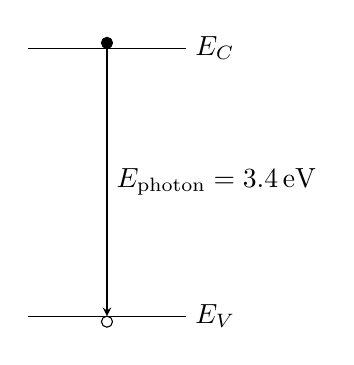
\begin{tikzpicture}
			\def\l{2};
			\def\eValence{1};
			\def\eConduction{\eValence + 3.4};

			\newcommand{\drawEnergyLevel}[1]
			{
				\draw (0,#1) -- (\l,#1)
			}

			\newcommand{\drawEnergyGap}[4]
			{
				\draw [|<->|] (#3,#1) -- (#3,#2) node [midway, left] {#4}
			}

			\begin{scope}
				\drawEnergyLevel{\eConduction} node [right] {$E_C$};
				\drawEnergyLevel{\eValence} node [right] {$E_V$};
			\end{scope}

			\begin{scope}
				\filldraw ($ (\l/2,\eConduction) + (0,2pt) $) circle (2pt);
				\draw ($ (\l/2,\eValence) - (0,2pt) $) circle (2pt);
			\end{scope}

			\begin{scope}[-stealth]
				\draw (\l/2,\eConduction) -- (\l/2,\eValence) node [midway, right] {$E_{\text{photon}} = 3.4 \electronvolt$};
			\end{scope}
		\end{tikzpicture}
		\caption{GaN : $E_g = 3.4 \electronvolt$}
	\end{figure}
	\begin{figure}[H]
		\centering
		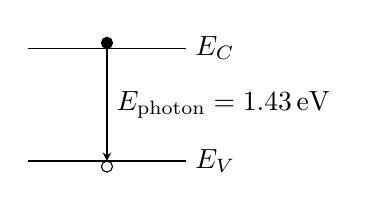
\begin{tikzpicture}
			\def\l{2};
			\def\eValence{1};
			\def\eConduction{\eValence + 1.43};

			\newcommand{\drawEnergyLevel}[1]
			{
				\draw (0,#1) -- (\l,#1)
			}

			\newcommand{\drawEnergyGap}[4]
			{
				\draw [|<->|] (#3,#1) -- (#3,#2) node [midway, left] {#4}
			}

			\begin{scope}
				\drawEnergyLevel{\eConduction} node [right] {$E_C$};
				\drawEnergyLevel{\eValence} node [right] {$E_V$};
			\end{scope}

			\begin{scope}
				\filldraw ($ (\l/2,\eConduction) + (0,2pt) $) circle (2pt);
				\draw ($ (\l/2,\eValence) - (0,2pt) $) circle (2pt);
			\end{scope}

			\begin{scope}[-stealth]
				\draw (\l/2,\eConduction) -- (\l/2,\eValence) node [midway, right] {$E_{\text{photon}} = 1.43 \electronvolt$};
			\end{scope}
		\end{tikzpicture}
		\caption{GaAs : $E_g = 1.43 \electronvolt$}
	\end{figure}
	\begin{figure}[H]
		\centering
		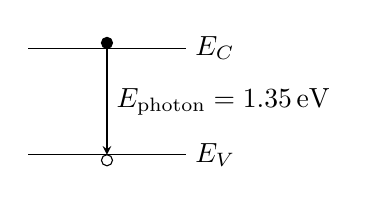
\begin{tikzpicture}
			\def\l{2};
			\def\eValence{1};
			\def\eConduction{\eValence + 1.35};

			\newcommand{\drawEnergyLevel}[1]
			{
				\draw (0,#1) -- (\l,#1)
			}

			\newcommand{\drawEnergyGap}[4]
			{
				\draw [|<->|] (#3,#1) -- (#3,#2) node [midway, left] {#4}
			}

			\begin{scope}
				\drawEnergyLevel{\eConduction} node [right] {$E_C$};
				\drawEnergyLevel{\eValence} node [right] {$E_V$};
			\end{scope}

			\begin{scope}
				\filldraw ($ (\l/2,\eConduction) + (0,2pt) $) circle (2pt);
				\draw ($ (\l/2,\eValence) - (0,2pt) $) circle (2pt);
			\end{scope}

			\begin{scope}[-stealth]
				\draw (\l/2,\eConduction) -- (\l/2,\eValence) node [midway, right] {$E_{\text{photon}} = 1.35 \electronvolt$};
			\end{scope}
		\end{tikzpicture}
		\caption{GaAs : $E_g = 1.35 \electronvolt$}
	\end{figure}
	\begin{enumerate}[leftmargin=*]
		\item For which materials will the emitted photon have the largest frequency?
			\begin{enumerate}
				\item GaN
				\item GaAs
				\item InP
			\end{enumerate}
		\item For which materials will the emitted photon have the largest wavelength?
			\begin{enumerate}
				\item GaN
				\item GaAs
				\item InP
			\end{enumerate}
		\item At room temperature, which material will have the maximum intrinsic carrier concentration $n_i$?
			\begin{enumerate}
				\item GaN
				\item GaAs
				\item InP
			\end{enumerate}
	\end{enumerate}
\end{question}

\begin{solution}
	\begin{enumerate}
		\item The emitted photon will have the largest frequency for \emph{GaN}.
		\item The emitted photon will have the largest wavelength for \emph{InP}.
		\item At room temperature, \emph{InP} will have the maximum intrinsic carrier concentration.
	\end{enumerate}
\end{solution}

\begin{question}
	Consider a sample of silicon that is doped with two donor levels $N_{D_1}$ donors per \si{\centi\metre\cubed} at donor energy $E_{D_1}$ with ionization energy 0.05 \electronvolt, and $N_{D_2}$ donors per \si{\centi\metre\cubed} at donor energy $E_{D_2}$ (deeper donor) with ionization energy 0.15 \electronvolt.
	\begin{enumerate}
		\item Draw the energy diagram for this material.
		\item Draw a graph of the electron concentration on a log scale as a function of $\frac{1}{T}$.
	\end{enumerate}
	Label the three regions of the plot, ionization, extrinsic, and intrinsic.
	On the graph, write the values of electron concentration in the extrinsic region.
\end{question}

\begin{solution}
	\begin{enumerate}[leftmargin=*]
		\item
			~\\
			\begin{figure}[H]
				\centering
				\begin{tikzpicture}[scale = 2]
					\def\l{2};
					\def\eValence{1};
					\def\eConduction{2};
					\def\eDOne{1.8};
					\def\eDTwo{1.6};
		
					\newcommand{\drawEnergyLevel}[1]
					{
						\draw (0,#1) -- (\l,#1)
					}
		
					\newcommand{\drawEnergyGap}[4]
					{
						\draw [|<->|] (#3,#1) -- (#3,#2) node [midway, left] {#4}
					}
		
					\begin{scope}
						\drawEnergyLevel{\eConduction} node [right] {$E_C$};
						\drawEnergyLevel{\eValence} node [right] {$E_V$};
						\drawEnergyLevel{\eDOne} node [right] {$E_{D_1}$};
						\drawEnergyLevel{\eDTwo} node [right] {$E_{D_2}$};
					\end{scope}
		
					\begin{scope}
						\drawEnergyGap{\eConduction}{\eDOne}{-1}{0.05 \electronvolt};
						\drawEnergyGap{\eConduction}{\eDTwo}{-2}{0.15 \electronvolt};
					\end{scope}
				\end{tikzpicture}
			\end{figure}
		\item 
			~\\
			\begin{figure}[H]
				\centering
				\begin{tikzpicture}
					\def\xMIN{0};
					\def\xMAX{10};
					\def\yMIN{0};
					\def\yMAX{9};
			
					\def\firstIntrinsicRegionThreshold{3};
					\def\interIntrinsicRegionThreshold{4};
					\def\secondIntrinsicRegionThreshold{5};
					\def\extrinsicRegionThreshold{7};
			
					\def\firstNd{4};
					\def\secondNd{3};
			
					\begin{scope}[-stealth]
						\draw (\xMIN,0) -- (\xMAX,0) node [right] {$\frac{1}{T}$ (\si{\per\kelvin})};
						\draw (0,\yMIN) -- (0,\yMAX) node [above] {$n$ (\si{\per\cubic\centi\meter}) (log scale)};
					\end{scope}
			
					\begin{scope}[dashed]
						\draw (\firstIntrinsicRegionThreshold,\yMIN) -- (\firstIntrinsicRegionThreshold,\yMAX);
						\draw (\interIntrinsicRegionThreshold,\yMIN) -- (\interIntrinsicRegionThreshold,\yMAX);
						\draw (\secondIntrinsicRegionThreshold,\yMIN) -- (\secondIntrinsicRegionThreshold,\yMAX);
						\draw (\extrinsicRegionThreshold,\yMIN) -- (\extrinsicRegionThreshold,\yMAX);
						\draw (\xMIN,\firstNd) node [left] {$N_{D_1} + N_{D_2}$} -- (\xMAX,\firstNd);
						\draw (\xMIN,\secondNd) node [left] {$N_{D_2}$} -- (\xMAX,\secondNd);
					\end{scope}
			
					\begin{scope}
						\draw [rounded corners = 10pt] ($ (\extrinsicRegionThreshold,\secondNd) + (2,-2) $) -- (\extrinsicRegionThreshold,\secondNd) -- (\secondIntrinsicRegionThreshold,\secondNd) -- (\interIntrinsicRegionThreshold,\firstNd) -- (\firstIntrinsicRegionThreshold,\firstNd) -- ++(-2,2);
					\end{scope}
			
					\begin{scope}
						\draw [decorate, decoration = {brace, mirror}, yshift = -10] (\xMIN,\yMIN) -- (\firstIntrinsicRegionThreshold,\yMIN) node [midway, below] {intrinsic};
						\draw [decorate, decoration = {brace, mirror}, yshift = -10] (\firstIntrinsicRegionThreshold,\yMIN) -- (\extrinsicRegionThreshold,\yMIN) node [midway, below] {extrinsic};
						\draw [decorate, decoration = {brace, mirror}, yshift = -10] (\extrinsicRegionThreshold,\yMIN) -- (\xMAX,\yMIN) node [midway, below] {ionization};
					\end{scope}

				\end{tikzpicture}
			\end{figure}
	\end{enumerate}
\end{solution}

\begin{question}
	\begin{enumerate}
		\item
			$\psi_1$ and $\psi_2$ are momentum eigenfunctions corresponding to different momentum eigenvalues, $p_1 \neq p_2$.
	Is $\psi = \psi_1 + \psi_2$ also a momentum eigenfunction?
			\begin{enumerate}
				\item Yes.
				\item No.
				\item It is impossible to answer based on the provided information.
			\end{enumerate}
		\item
			Two particles, 1 and 2, are described by plane waves of the form $e^{i k x}$.
			Particle 1 is described by a smaller wavelength than particle 2, $\lambda_1 < \lambda_2$.
			Which particle has a larger momentum?
			\begin{enumerate}
				\item Particle 1.
				\item Particle 2.
				\item Both have the same momentum.
				\item It is impossible to answer based on the provided information.
			\end{enumerate}
		\item
			Consider the eigenvalue equation
			\begin{align*}
				\dod[2]{}{x}f(x) & = c f(x)
			\end{align*}
			How many of the following give an eigenfunction and a corresponding eigenvalue to the above equation?
			\begin{enumerate}
				\item $f(x) = sin(k x)$, $c = k^2$
				\item $f(x) = e^{-x}$, $c = 1$
				\item $f(x) = e^{i k x}$, $c = -k^2$
				\item $f(x) = x^3$, $c = 6$
			\end{enumerate}
			\begin{enumerate}
				\item 1
				\item 2
				\item 3
				\item 4
				\item none
			\end{enumerate}
	\end{enumerate}
\end{question}

\begin{solution}
	\begin{enumerate}[leftmargin=*]
		\item
			Let
			\begin{align*}
				\psi_1 & = A_1 e^{i k_1 x} \\
				\psi_2 & = A_2 e^{i k_2 x}
			\end{align*}
			Therefore,
			\begin{align*}
				\frac{\hbar}{i} \dpd{}{x}\left( \psi_1 + \psi_2 \right) & = \frac{\hbar}{i} \dpd{}{x}\left( A_1 e^{i k_1 x} + A_2 e^{i k_2 x} \right) \\
                                                                                        & = \frac{\hbar}{i} i k_1 \psi_1 + i k_2 \psi_2                               \\
                                                                                        & \neq c \left( \psi_1 + \psi_2 \right)
			\end{align*}
			Therefore, \emph{$\psi = \psi_1 + \psi_2$ is not a momentum eigenfunction}.
		\item
			According to the de Broglie hypothesis,
			\begin{align*}
				p & = \frac{h}{\lambda}
			\end{align*}
			Therefore, as $\lambda_1 < \lambda_2$, $p_1 > p_2$.
			Hence, \emph{particle 1} has larger momentum.
		\item
			\begin{align*}
				\dod[2]{}{x} f(x) & = c f(x)
			\end{align*}
			Therefore,
			\begin{align*}
				\dod[2]{\sin(k x)}{x} & = c \sin(k x) \\
				-\sin(k^2 x)          & = c \sin(k x)
			\end{align*}
			Therefore, \emph{$c = k^2$ is not an eigenvalue} of the function.\\
			~\\
			\begin{align*}
				\dod[2]{}{x} f(x) & = c f(x)
			\end{align*}
			Therefore,
			\begin{align*}
				\dod[2]{e^{-x}} e^{-x} & = c e^{-x} \\
				\therefore e^{-x}      & = c e^{-x}
			\end{align*}
			Therefore, \emph{$c = 1$ is an eigenvalue} of the function.\\
			~\\
			\begin{align*}
				\dod[2]{}{x} f(x) & = c f(x)
			\end{align*}
			Therefore,
			\begin{align*}
				\dod[2]{}{x} e^{i k x}    & = c e^{i k x} \\
				\therefore -k^2 e^{i k x} & = c e^{i k x}
			\end{align*}
			Therefore, \emph{$c = -k^2$ is an eigenvalue} of the function.\\
			~\\
			\begin{align*}
				\dod[2]{}{x} f(x) & = c f(x)
			\end{align*}
			Therefore,
			\begin{align*}
				\dod[2]{x^3}{x} & = c x^3 \\
				6 x             & = c x^3
			\end{align*}
			Therefore, \emph{$c = 6$ is not an eigenvalue} of the function.
	\end{enumerate}
	Hence, \emph{2} of the pairs are pairs of eigenvalues and eigenfunctions.
\end{solution}

\begin{question}
		A particle is represented, at time $t=0$ by the following wave function:
		\begin{align*}
			\psi(x,0) &=
				\begin{cases}
					A \left( a^2 - x^2 \right) & ;\quad -a \le x \le a \\
					0                          & ;\quad \text{otherwise}
				\end{cases}
		\end{align*}
		\begin{enumerate}
			\item Find $\sigma_x$, the uncertainty in $x$.
			\item Find $\sigma_p$, the uncertainty in $p$.
			\item Check if your results are consistent with the uncertainty principle.
		\end{enumerate}
\end{question}

\begin{solution}
	\begin{enumerate}[leftmargin=*]
		\item
			\begin{align*}
				\sigma_x & = \sqrt{\left\langle x^2 \right\rangle - \langle x \rangle^2} \\
                                         & = \sqrt{\frac{1}{7} a^2}                                      \\
                                         & = \frac{a}{\sqrt{7}}
			\end{align*}
		\item
			\begin{align*}
				\sigma_p & = \sqrt{\left\langle p^2 \right\rangle - \langle p \rangle^2} \\
                                         & = \sqrt{\frac{5 h^2}{2 a^2}}                                  \\
                                         & = \sqrt{\frac{5}{2}} \frac{h}{a}
			\end{align*}
		\item
			\begin{align*}
				\sigma_x \sigma_p & = \frac{a}{\sqrt{7}} \sqrt{\frac{5}{2}} \frac{h}{a} \\
                                                  & = \sqrt{\frac{5}{14}} h                             \\
                                                  & = \frac{h}{2} \sqrt{\frac{10}{7}}                   \\
                                                  & > \frac{h}{2}
			\end{align*}
			Therefore, the results are consistent with the uncertainty principle.
	\end{enumerate}
\end{solution}

\begin{question}
	Consider a particle described by a certain wave function $\psi(x)$, and an observable $A$, associated with operator $\hat{A}$.\\
	Determine whether the following statements are true or false, and explain your answer.
	\begin{enumerate}
		\item The two following actions are identical and give the same result - measuring observable $A$ for this state $\psi(x)$ and applying the operator $\hat{A}$ on $\psi(x)$.
		\item Measuring observable $A$ and applying the operator $\hat{A}$ on $\psi(x)$ both cause a collapse of the wave function.
		\item Measuring observable $A$ always returns an eigenvalue of operator $\hat{A}$.
	\end{enumerate}
\end{question}

\begin{solution}
	\begin{enumerate}[leftmargin=*]
		\item
			False.
			When an observable is measured, the result is an eigenvalue of the operator corresponding to the observable.
			When an operator is applied to the wave function, the result is a function.
		\item
			False, as the wave function collapses only on physical measurement of the particle, only the process of measuring $A$ causes the collapse, while the process of applying the operator in the wave function does not.
		\item
			True
	\end{enumerate}
\end{solution}

\end{document}
